\documentclass{beamer}
\usepackage[utf8]{inputenc}
\usepackage{setspace}
\usepackage{hyperref}
\usepackage{amsmath}
\usepackage{pifont}
\usepackage{color}
% Just add % Just add % Just add \input{smalltalkEnv} to your file
% then you can use :
% \begin{lstlisting}[language=Smalltalk]
% false become: true.
% \end{lstlisting}

\usepackage{color}
\usepackage{listings}
\usepackage{etoolbox}
\usepackage{textcomp}

\definecolor{stComment}{rgb}{0.5,0.5,0.5}
\definecolor{stString}{rgb}{0.58,0,0.82}
\definecolor{stKeywords}{rgb}{0.21,0.55,0.7}
\definecolor{stNumbers}{rgb}{.5,0,0}

\newtoggle{InString}{}% Keep track of if we are within a string
\togglefalse{InString}% Assume not initally in string
\newcommand*{\ColorIfNotInString}[1]{\iftoggle{InString}{#1}{\color{stNumbers}#1}}%
\newcommand*{\ProcessQuote}[1]{#1\iftoggle{InString}{\global\togglefalse{InString}}{\global\toggletrue{InString}}}%

\lstdefinelanguage{Smalltalk}{
  keywordstyle=\color{stKeywords},
  commentstyle=\color{stComment},
  stringstyle=\color{stString},
  alsoletter=\#,
  identifierstyle=\idstyle, 
  showstringspaces=false,
  morekeywords={true,false,self,super,nil},
  sensitive=true, 
  morecomment=[s]{"}{"}, 
  morestring=[d]', 
  style=SmalltalkStyle,
  tabsize=2,
  basicstyle=\ttfamily,
  upquote=true,
}


\makeatletter%
\newcommand*\idstyle[1]{%
  \expandafter\id@style\the\lst@token{#1}\relax%
}
\def\id@style#1#2\relax{%
  \ifnum\pdfstrcmp{#1}{\#}=0%
  \ttfamily\color{stString} \the\lst@token%
  \else%
  \edef\tempa{\uccode`#1}%
  \edef\tempb{`#1}%
  \ifnum\tempa=\tempb%
  \ttfamily\color{blue} \the\lst@token%
  \else%
  \the\lst@token%
  \fi%
  \fi%
}

\lstdefinestyle{SmalltalkStyle}{ 
  literate=%
  {^}{{$\uparrow$}}1% 
  % {"}{{{\ProcessQuote{"}}}}1% Disable coloring within double quotes
  % {'}{{{\ProcessQuote{'}}}}1% Disable coloring within single quote
  {0}{{{\ColorIfNotInString{0}}}}1%
  {1}{{{\ColorIfNotInString{1}}}}1%
  {2}{{{\ColorIfNotInString{2}}}}1%
  {3}{{{\ColorIfNotInString{3}}}}1%
  {4}{{{\ColorIfNotInString{4}}}}1%
  {5}{{{\ColorIfNotInString{5}}}}1%
  {6}{{{\ColorIfNotInString{6}}}}1%
  {7}{{{\ColorIfNotInString{7}}}}1%
  {8}{{{\ColorIfNotInString{8}}}}1%
  {9}{{{\ColorIfNotInString{9}}}}1%
} 
 to your file
% then you can use :
% \begin{lstlisting}[language=Smalltalk]
% false become: true.
% \end{lstlisting}

\usepackage{color}
\usepackage{listings}
\usepackage{etoolbox}
\usepackage{textcomp}

\definecolor{stComment}{rgb}{0.5,0.5,0.5}
\definecolor{stString}{rgb}{0.58,0,0.82}
\definecolor{stKeywords}{rgb}{0.21,0.55,0.7}
\definecolor{stNumbers}{rgb}{.5,0,0}

\newtoggle{InString}{}% Keep track of if we are within a string
\togglefalse{InString}% Assume not initally in string
\newcommand*{\ColorIfNotInString}[1]{\iftoggle{InString}{#1}{\color{stNumbers}#1}}%
\newcommand*{\ProcessQuote}[1]{#1\iftoggle{InString}{\global\togglefalse{InString}}{\global\toggletrue{InString}}}%

\lstdefinelanguage{Smalltalk}{
  keywordstyle=\color{stKeywords},
  commentstyle=\color{stComment},
  stringstyle=\color{stString},
  alsoletter=\#,
  identifierstyle=\idstyle, 
  showstringspaces=false,
  morekeywords={true,false,self,super,nil},
  sensitive=true, 
  morecomment=[s]{"}{"}, 
  morestring=[d]', 
  style=SmalltalkStyle,
  tabsize=2,
  basicstyle=\ttfamily,
  upquote=true,
}


\makeatletter%
\newcommand*\idstyle[1]{%
  \expandafter\id@style\the\lst@token{#1}\relax%
}
\def\id@style#1#2\relax{%
  \ifnum\pdfstrcmp{#1}{\#}=0%
  \ttfamily\color{stString} \the\lst@token%
  \else%
  \edef\tempa{\uccode`#1}%
  \edef\tempb{`#1}%
  \ifnum\tempa=\tempb%
  \ttfamily\color{blue} \the\lst@token%
  \else%
  \the\lst@token%
  \fi%
  \fi%
}

\lstdefinestyle{SmalltalkStyle}{ 
  literate=%
  {^}{{$\uparrow$}}1% 
  % {"}{{{\ProcessQuote{"}}}}1% Disable coloring within double quotes
  % {'}{{{\ProcessQuote{'}}}}1% Disable coloring within single quote
  {0}{{{\ColorIfNotInString{0}}}}1%
  {1}{{{\ColorIfNotInString{1}}}}1%
  {2}{{{\ColorIfNotInString{2}}}}1%
  {3}{{{\ColorIfNotInString{3}}}}1%
  {4}{{{\ColorIfNotInString{4}}}}1%
  {5}{{{\ColorIfNotInString{5}}}}1%
  {6}{{{\ColorIfNotInString{6}}}}1%
  {7}{{{\ColorIfNotInString{7}}}}1%
  {8}{{{\ColorIfNotInString{8}}}}1%
  {9}{{{\ColorIfNotInString{9}}}}1%
} 
 to your file
% then you can use :
% \begin{lstlisting}[language=Smalltalk]
% false become: true.
% \end{lstlisting}

\usepackage{color}
\usepackage{listings}
\usepackage{etoolbox}
\usepackage{textcomp}

\definecolor{stComment}{rgb}{0.5,0.5,0.5}
\definecolor{stString}{rgb}{0.58,0,0.82}
\definecolor{stKeywords}{rgb}{0.21,0.55,0.7}
\definecolor{stNumbers}{rgb}{.5,0,0}

\newtoggle{InString}{}% Keep track of if we are within a string
\togglefalse{InString}% Assume not initally in string
\newcommand*{\ColorIfNotInString}[1]{\iftoggle{InString}{#1}{\color{stNumbers}#1}}%
\newcommand*{\ProcessQuote}[1]{#1\iftoggle{InString}{\global\togglefalse{InString}}{\global\toggletrue{InString}}}%

\lstdefinelanguage{Smalltalk}{
  keywordstyle=\color{stKeywords},
  commentstyle=\color{stComment},
  stringstyle=\color{stString},
  alsoletter=\#,
  identifierstyle=\idstyle, 
  showstringspaces=false,
  morekeywords={true,false,self,super,nil},
  sensitive=true, 
  morecomment=[s]{"}{"}, 
  morestring=[d]', 
  style=SmalltalkStyle,
  tabsize=2,
  basicstyle=\ttfamily,
  upquote=true,
}


\makeatletter%
\newcommand*\idstyle[1]{%
  \expandafter\id@style\the\lst@token{#1}\relax%
}
\def\id@style#1#2\relax{%
  \ifnum\pdfstrcmp{#1}{\#}=0%
  \ttfamily\color{stString} \the\lst@token%
  \else%
  \edef\tempa{\uccode`#1}%
  \edef\tempb{`#1}%
  \ifnum\tempa=\tempb%
  \ttfamily\color{blue} \the\lst@token%
  \else%
  \the\lst@token%
  \fi%
  \fi%
}

\lstdefinestyle{SmalltalkStyle}{ 
  literate=%
  {^}{{$\uparrow$}}1% 
  % {"}{{{\ProcessQuote{"}}}}1% Disable coloring within double quotes
  % {'}{{{\ProcessQuote{'}}}}1% Disable coloring within single quote
  {0}{{{\ColorIfNotInString{0}}}}1%
  {1}{{{\ColorIfNotInString{1}}}}1%
  {2}{{{\ColorIfNotInString{2}}}}1%
  {3}{{{\ColorIfNotInString{3}}}}1%
  {4}{{{\ColorIfNotInString{4}}}}1%
  {5}{{{\ColorIfNotInString{5}}}}1%
  {6}{{{\ColorIfNotInString{6}}}}1%
  {7}{{{\ColorIfNotInString{7}}}}1%
  {8}{{{\ColorIfNotInString{8}}}}1%
  {9}{{{\ColorIfNotInString{9}}}}1%
} 

\usetheme{AnnArbor}

% My preferences
\graphicspath{{images/}}
\newcommand{\tip}{\boldmath{\textcolor{red}{$\Rightarrow$}}}
\newcommand{\drgeo}{Dr.~Geo}
\newcommand{\cmark}{\text{\ding{51}}}
\newcommand{\xmark}{\text{\ding{55}}}

\title{Revisiting the Dynabook concept}

\author{Hilaire Fernandes}
\institute[DIP, Geneva]{Department of Public Instruction \\ Geneva}
\titlegraphic{
  
\includegraphics[width=2cm]{ArmoirieGeneve.png}
}
\date{November 2023}

\begin{document}
\begin{frame}
  \titlepage
\end{frame}
%
\begin{frame}{About me}
  \fontsize{12pt}{30pt}\selectfont
  \begin{itemize}
  \item Educator in public school, Geneva, B.Math, Ma.Ed
  \item Computer scientist, Ma.CS, PhD.CS
  \item Free software enthusiast and user since 1998
  \item And of course, Smalltalk user since 2002
  \end{itemize}
\end{frame}
%
\begin{frame}{Contents}
  \tableofcontents[hideallsubsections]
\end{frame}

\section{Why this presentation?}

\begin{frame}{Cashier machine for education}
  \begin{itemize}
  \item The Dynabook is still only a concept
  \item In school, dynamic numeric tool mostly not used\\
    \tip\ observe the other sectors of the society
\end{itemize}
\end{frame}
%
\begin{frame}{To get you involved}
  \begin{itemize}
  \item Educator, professor
  \item Benefactor
  \item Student at university
  \item Econimist
  \item Software developer
  \item Project manager
  \item Hardware specialist
  \item Designer
  \item System administrator
  \item ...
  \end{itemize}
\end{frame}

\section{In essence, what is Dynabook?}
\begin{frame}
  \fontsize{14pt}{8pt}\selectfont
\begin{center}
  Dynamic model of knowledge\\ the learner can operate on
\end{center}
\end{frame}
%
\begin{frame}{Dynamic model of the \emph{Newton Telescop}}
 The learner
  can operate a different level of knowledge light beam, focus point
  (change the mirror curve)
\begin{center}
  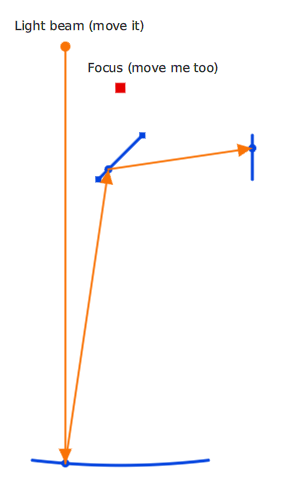
\includegraphics[width=0.3\textwidth]{Newton.png}
\end{center}
\end{frame}

\section{Changing the Point of View}
\begin{frame}{Teacher}
  What is a teacher?
  \vspace*{10pt}
  \begin{itemize}
  \item Yes, an educator. Manipulating, designing, sharing knowledge.\\
    \tip\ Library of dynamic knowledge models, scriptable with a DSL
    and/or GUI (think \drgeo)

  \item ... but also a manager
    \begin{itemize}
    \item managing student
    \item managing assignment
    \item managing grade
    \item managing meeting
    \item managing parents
    \item ...
    \end{itemize}
  \end{itemize}
  \vspace*{10pt}

  Any realistic Dynabook revisit should take theses aspects in
  consideration.
\end{frame}
%
\begin{frame}{Kid}
  Can we reduce the bag wight?

  \vspace*{10pt}

  I have seen lightweight students assigned with mountain of materials:
  \begin{itemize}
  \item $>$10 binders
  \item $>$10 books
  \item $>$10 activity files
  \item numerous notebooks
  \end{itemize}

  \vspace*{10pt}
  
  Any realistic Dynabook revisit should take theses aspects in
  consideration.

\end{frame}
%
\begin{frame}{Software environment}
  What do we need?

  \vspace{10pt}
  
  \begin{itemize}
  \item Free software from the basement (OS) to the attic (end user
    applications)
  \item Rapid prototyping
  \item A malleable environment to develop knowledge models with state
    of the art visual representation
  \item Easy to implement DSL to script knowledge models
  \item Portable to different hardware architecture
  \end{itemize}

  \vspace*{10pt}

  \tip\ Cuis-Smalltalk to develop end user applications and knowledge
  models
\end{frame}
%
\begin{frame}{Free Hardware}
  \fontsize{14pt}{8pt}\selectfont
  \begin{center}
    Design there\\
    \vspace*{10pt}
    Manufacture anywhere
  \end{center}
\end{frame}

\begin{frame}{Economic}
  Large scale adoption in one place, also require local economic
  benefit on that place:
  \begin{itemize}
  \item Software support
  \item Assembling/Manufacturing
  \item Repairing
  \item Training
  \end{itemize}

  \vspace*{10pt}
  
  \tip\ Free software \& hardware as prerequisites
  
\end{frame}

\section{Where are we?}
\begin{frame}{Is there any plan?}
\begin{center}
  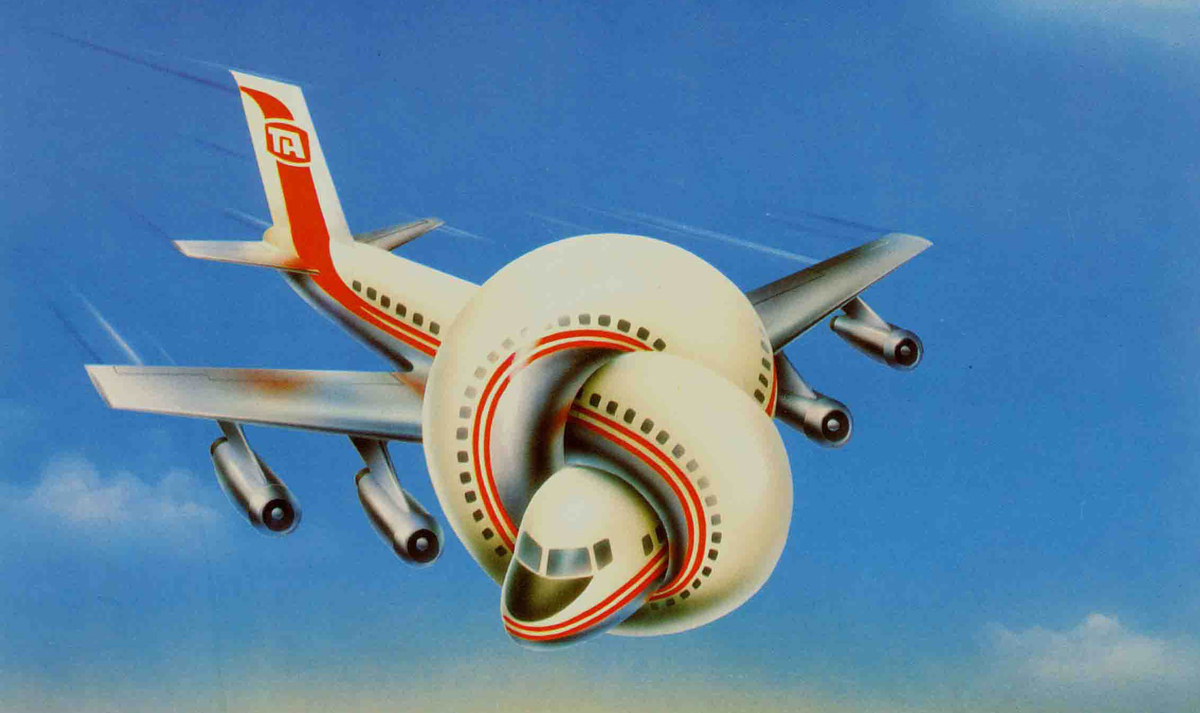
\includegraphics[width=0.8\textwidth]{anyPilot.jpeg}
\end{center}
\end{frame}
\begin{frame}{Roughly}
  Iterations
  \begin{enumerate}
  \item \textbf{Develop the Dynabook app} (me, but join!)
  \item Test Dynabook app in school and iterate with the development (1 or 2 users)
  \item Develop hardware prototype with existing hardware
  \item Develop Dynabook operating system
  \item Test Dynabook app in school and iterate with the development (tenth of users)
  \item Test Dynabook in school and iterate on the hardware and software (1 or 2 users)
  \item Test Dynabook hardware and software with one classroom (30 users, students and teachers)
  \end{enumerate}
\end{frame}

\begin{frame}{Visual Concepts}
  
\end{frame}


\section{How to get involved?}

\end{document}